\section{Results}
\label{sec:results}

\subsection{Main Comparison: Execution vs.\ Pylint/Mypy (RQ1)}

Execution feedback significantly outperforms pylint/mypy feedback on both benchmarks. Figure~\ref{fig:delta} shows the pass@1 improvement delta with 95\% bootstrap confidence intervals.

\begin{table}[h]
\centering
\caption{Main results: pass@1 and improvement delta ($\Delta$) per condition.}
\label{tab:main}
\begin{tabular}{lllll}
\toprule
\textbf{Condition} & \textbf{HE pass@1} & \textbf{$\Delta_{\text{HE}}$} & \textbf{MBPP pass@1} & \textbf{$\Delta_{\text{MBPP}}$} \\
\midrule
No-feedback (baseline) & 61.0\% & --- & 33.1\% & --- \\
Pylint/mypy repair & 56.7\% & $-$4.3pp & 51.4\% & +18.3pp \\
Execution feedback & 65.9\% & \textbf{+4.9pp} & 73.3\% & \textbf{+40.2pp} \\
\bottomrule
\end{tabular}
\end{table}

The most striking result is on MBPP: a single round of execution feedback repair improves pass@1 from 33.1\% to 73.3\%---a +40.2pp absolute improvement, more than doubling the baseline success rate.

\begin{table}[h]
\centering
\caption{McNemar test results: problems exclusively repaired by each condition.}
\label{tab:mcnemar}
\begin{tabular}{llll}
\toprule
\textbf{Benchmark} & \textbf{Exec-only} & \textbf{Pylint-only} & \textbf{McNemar $p$-value} \\
\midrule
HumanEval & 15 & 0 & $p$ = 0.0001 \\
MBPP & 85 & 2 & $p$ < 10$^{-18}$ \\
\bottomrule
\end{tabular}
\end{table}

On HumanEval, 15 problems are exclusively repaired by execution feedback---zero are exclusively repaired by pylint. On MBPP, 85 problems are exclusively repaired by execution vs.\ 2 by pylint.

\begin{figure}[h]
\centering
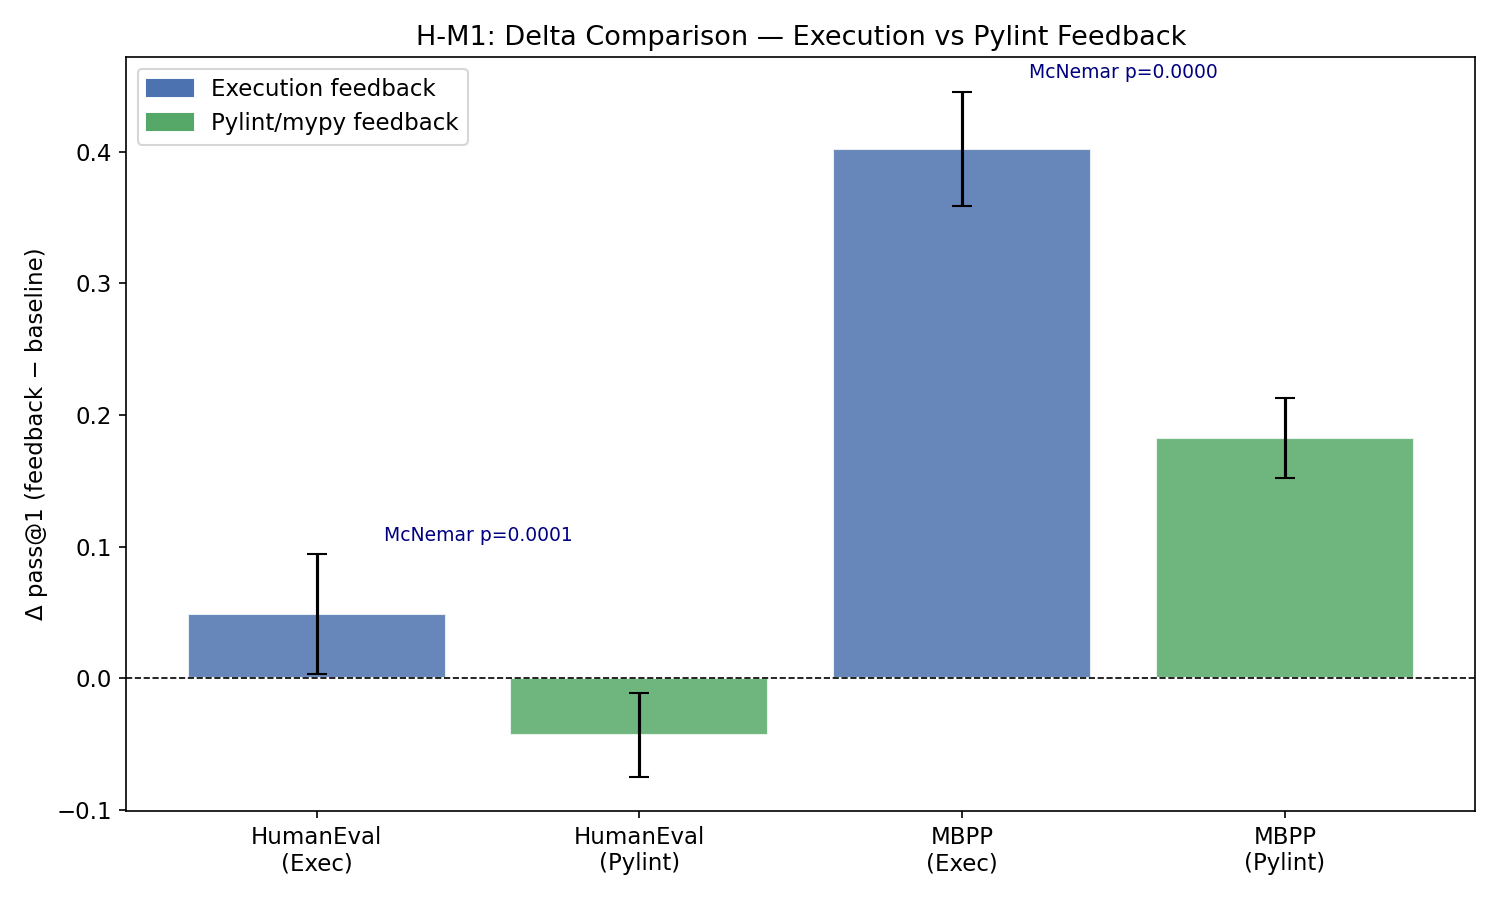
\includegraphics[width=0.85\columnwidth]{figures/figure1_delta_comparison.png}
\caption{Pass@1 improvement delta ($\Delta$) with 95\% bootstrap CIs and McNemar $p$-values for both benchmarks. Execution feedback (blue) significantly outperforms pylint/mypy (orange) on both HumanEval and MBPP.}
\label{fig:delta}
\end{figure}

\begin{figure}[h]
\centering
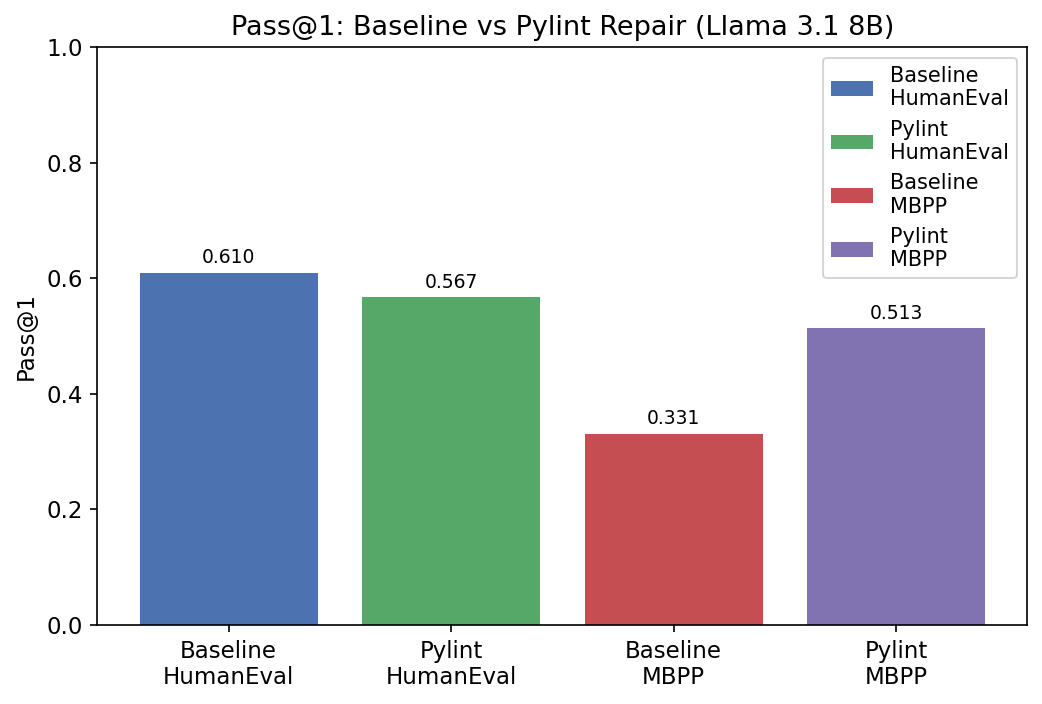
\includegraphics[width=0.85\columnwidth]{figures/figure1_pass_at_1_comparison.png}
\caption{Absolute pass@1 values for all three conditions on both benchmarks.}
\label{fig:absolute}
\end{figure}

\subsection{Pylint/Mypy Coverage Analysis---The Mechanism (RQ2)}

\textbf{Coverage result:} Pylint/mypy flags 100\% of the 64 HumanEval baseline failures (bootstrap CI: [100\%, 100\%]).

\begin{table}[h]
\centering
\caption{Pylint flag category distribution across 64 HumanEval failures (300 total flags).}
\label{tab:pylint}
\begin{tabular}{lllll}
\toprule
\textbf{Category} & \textbf{Flags} & \textbf{Fraction} & \textbf{Type} \\
\midrule
C (Convention) & 283 & 94.3\% & Style (C0304, C0114) \\
R (Refactor) & 8 & 2.7\% & Style/structure \\
W (Warning) & 7 & 2.3\% & Functional \\
E (Error) & 1 & 0.3\% & Functional \\
I (Information) & 1 & 0.3\% & Informational \\
\bottomrule
\end{tabular}
\end{table}

\textbf{Functional coverage (E+W):} 8/64 failures = 12.5\% (8 distinct failures receiving at least one Error or Warning flag; the single I-category flag is informational, not functional). Mypy coverage: 0/64 = 0\%.

The 100\% total coverage is driven by C0304 (``missing newline at end of file'') and C0114 (``missing docstring in public module'')---properties of LLM code generation context, not indicators of logical errors.

\begin{figure}[h]
\centering
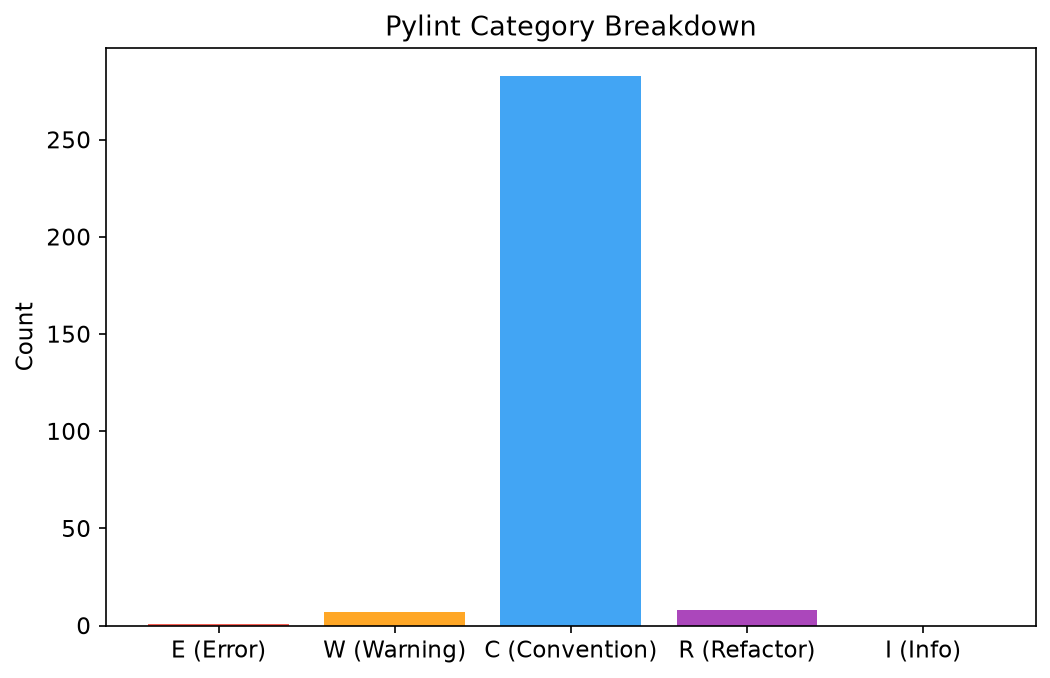
\includegraphics[width=0.85\columnwidth]{figures/fig2_pylint_categories.png}
\caption{Pylint flag category distribution across 64 HumanEval failures. The 94.3\% Convention-category dominance (C0304, C0114) reveals the style-function dissociation: pylint's high coverage is driven by style rules orthogonal to functional correctness.}
\label{fig:categories}
\end{figure}

\begin{figure}[h]
\centering
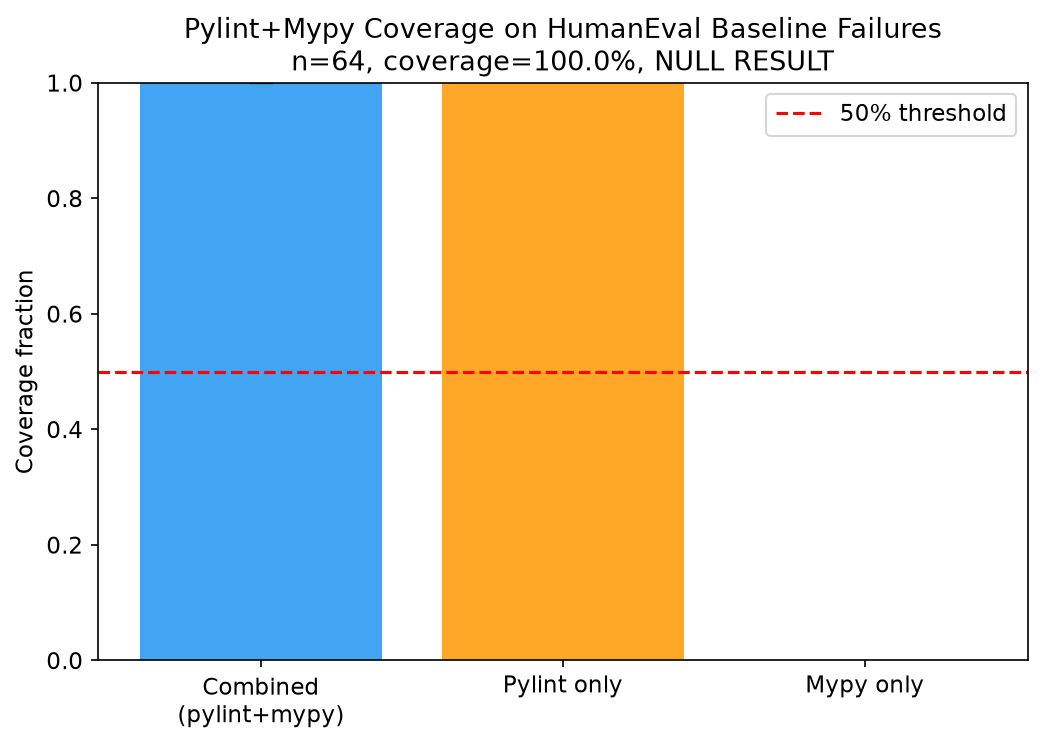
\includegraphics[width=0.85\columnwidth]{figures/fig1_coverage_bar.png}
\caption{Total pylint/mypy coverage (100\%) vs.\ functional coverage (E+W only, 12.5\%) with 95\% bootstrap confidence intervals across HumanEval baseline failures.}
\label{fig:coverage}
\end{figure}

\subsection{Benchmark Asymmetry and Task-Complexity Moderation (RQ3)}

Pylint repair hurts HumanEval ($-$4.3pp) but helps MBPP (+18.3pp). We interpret this as task-complexity moderation: MBPP's simpler function-completion tasks tolerate style-guided rewrites without losing logical structure; HumanEval's algorithmic problems are sensitive to rewriting triggered by style feedback.

\begin{figure}[h]
\centering
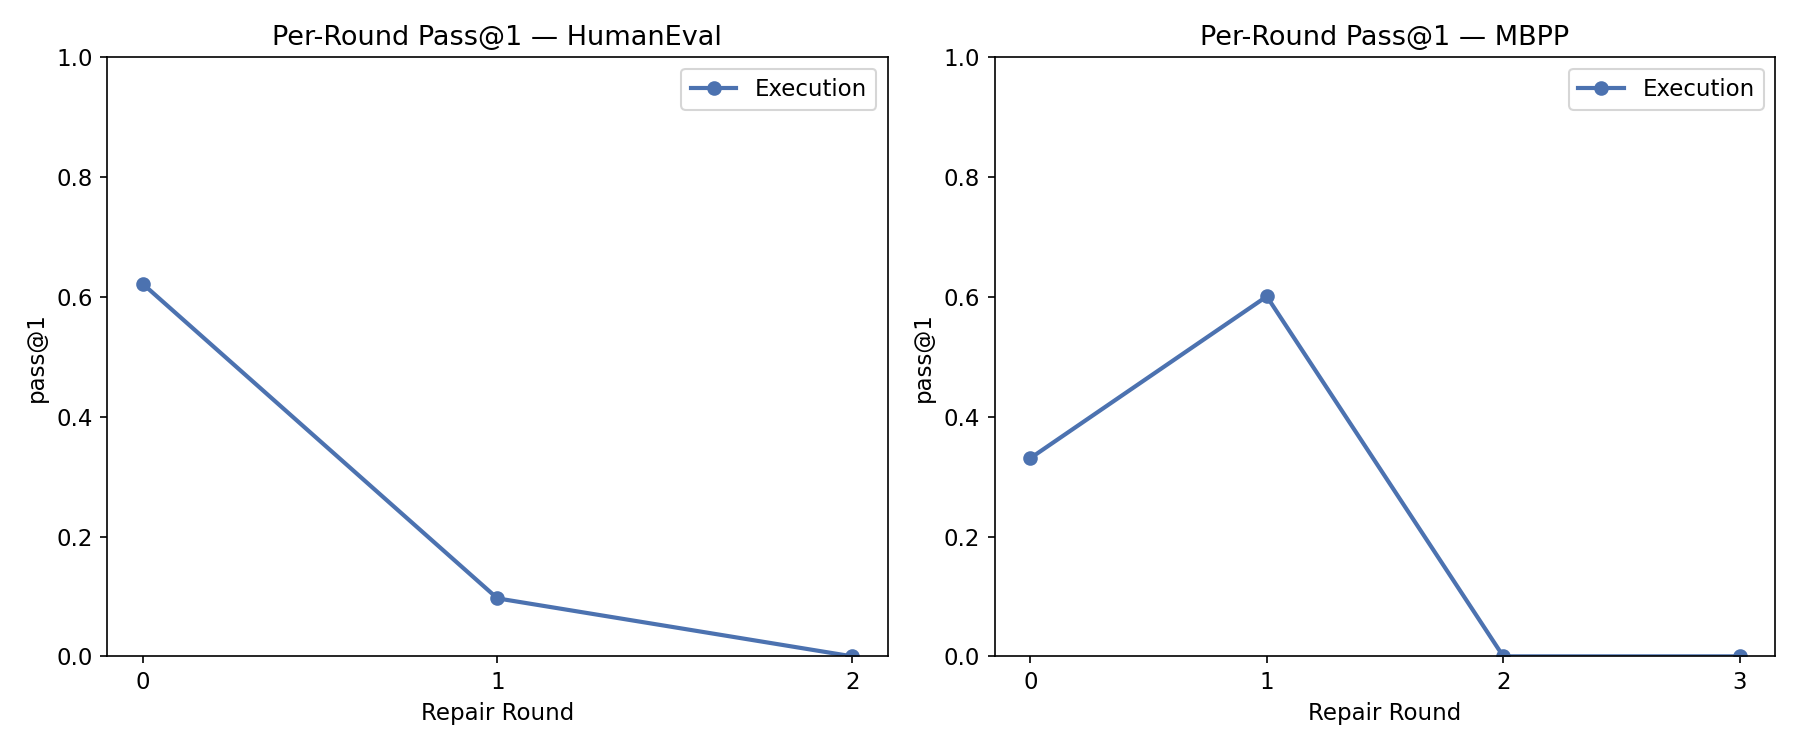
\includegraphics[width=0.85\columnwidth]{figures/figure2_per_round_trajectory.png}
\caption{Per-round pass@1 trajectory (rounds 0--3) for execution feedback condition, confirming round-1 dominance at $B$=1000.}
\label{fig:trajectory}
\end{figure}

\subsection{Budget Saturation}

At $B$=1000, the token budget is effectively exhausted after round 1 for most problems. Figure~\ref{fig:trajectory} confirms that rounds 2--3 contribute near-zero incremental improvement. Results characterize \textbf{single-round repair at $B$=1000}. Note: Round 0 in Figure~\ref{fig:trajectory} represents the initial generation pass@1 within the execution feedback condition's experimental run and may differ slightly from the no-feedback baseline (61.0\%) due to prompt-context differences; the no-feedback baseline is a separate single-pass condition without any repair loop instrumentation.
